\documentclass[11pt]{article}

\usepackage[a4paper,margin=1in]{geometry}
\usepackage{amsmath}
\usepackage{graphicx}
\usepackage{booktabs}
\usepackage{subcaption}
\usepackage{microtype}
\usepackage{titlesec}
\usepackage{xcolor}
\usepackage{caption}
\usepackage[hidelinks]{hyperref}
\usepackage{enumitem}

\graphicspath{{../figures/}{../figures/pages/}}

\definecolor{accent}{HTML}{7A1F2B}
\captionsetup{font=small,labelfont={bf,color=accent}}
\titleformat{\section}{\large\bfseries\color{accent}}{\thesection}{0.6em}{}
\titleformat{\subsection}{\normalsize\bfseries}{\thesubsection}{0.6em}{}

\setlength{\parskip}{0.35em}
\setlength{\parindent}{0pt}

\newcommand{\tw}{\ensuremath{\tau}}

\title{\vspace{-2.2em}\bfseries Detection is easy, reading order is the tax\\[0.35em]
\large\mdseries A multilingual benchmark of line detection and reading order\\
on historical documents}

\author{Abhishek Jha\\[0.2em]
\small Independent researcher\\
\small \href{https://huggingface.co/abhishekjha1008}{huggingface.co/abhishekjha1008} \;\textperiodcentered\;
\href{https://github.com/AbhiPandit1}{github.com/AbhiPandit1}}

\date{\small Working draft, September 2026}

\begin{document}
\maketitle
\thispagestyle{empty}

\begin{abstract}
\noindent
On historical documents, finding the text lines on a page is close to solved;
deciding the \emph{order} in which to read them is not. On a single column the two
questions collapse into one, so the reading-order problem stays hidden until the
layout has more than one column. We benchmark five widely used segmentation
systems --- kraken, a domain-adapted YOLOv8 line detector, Surya, docTR and
Tesseract --- on 40 pages across eight languages and roughly four centuries,
scoring each on two separate quantities: line-detection F at IoU $\ge 0.5$, and a
reading-order Kendall \tw{} between the predicted order and the ground-truth
document order, measured only on the lines that were actually detected. The pure
box detectors match the purpose-built segmenter on detection (F $0.91$ each) but
collapse on reading order for multi-column pages (\tw{} $\approx 0.5$, close to
random), while layout-aware systems hold \tw{} $\approx 0.97$--$1.00$. The effect
is confined to multi-column layouts and is \emph{era-invariant}: it appears
identically on a seventeenth-century Swedish handwritten court record and a
twentieth-century printed English page. We then show that the gap is not
intrinsic to fast detectors: adding a cheap column-clustering ordering stage on
top of the same detected boxes raises multi-column \tw{} from $0.50$ to $0.99$
(95\% CI $[0.98,1.00]$), statistically indistinguishable from the layout-aware
segmenter, at roughly nine times the speed. A downstream analysis makes the stake
concrete: assuming perfect line recognition, naive ordering alone inflicts a
median $82\%$ word error on multi-column pages, which the ordering stage cuts to
$2\%$. We argue that reading order should be reported as a first-class metric
alongside recognition accuracy, and release the data, ground truth, predictions
and a reproducible harness.
\end{abstract}

\section{Introduction}

Most published Handwritten Text Recognition (HTR) and OCR results report Character
Error Rate (CER) on lines that have already been cut out and placed in the correct
reading order, whether produced by end-to-end toolchains such as
Transkribus~\cite{transkribus} and kraken~\cite{kraken} or by neural line
recognisers~\cite{pylaia}. This hides a large part of real-world error. When a page has
columns, marginalia or tabular structure, the step that decides \emph{in what
order} the detected lines are fed to the recogniser determines whether the final
transcription is usable at all: a perfect line-level transcription, emitted in the
wrong order, still yields scrambled text.

The reason this is easy to overlook is that on a single-column page detection and
ordering are the same problem --- a top-to-bottom sort of the detected lines is
already the correct reading order. The difficulty only becomes visible when the
layout branches. This paper isolates that difficulty. We take the same set of
historical pages and ask each segmentation system two questions that are usually
conflated: \textbf{did you find the lines?} and \textbf{did you read them in the
right order?} We find that modern detectors have largely solved the first and that
the second is where systems still diverge sharply --- but only on multi-column
material.

\section{Related work}

\textbf{Layout analysis and line detection.} Historical page segmentation is
served by neural systems such as kraken's \texttt{blla}~\cite{kraken}, Laypa
(used in the Loghi pipeline), dhSegment~\cite{dhsegment} and eynollah, and by
baseline-detection methods evaluated in the cBAD competitions~\cite{cbad}.
General object detectors such as YOLO~\cite{yolov8} have been adapted to line
detection with strong results. These systems are typically scored on region or
baseline overlap; the order their output implies is rarely evaluated separately.

\textbf{Reading-order determination.} Ordering detected regions has a long
history, from recursive XY-cut~\cite{xycut} and topological or graph-based
sorting to learned approaches: LayoutReader~\cite{layoutreader} casts reading
order as a sequence-to-sequence problem over layout tokens. Most such work
targets modern printed documents (forms, scientific papers) where ground-truth
reading order is abundant; early-modern manuscript pages with multi-column and
marginal structure are far less studied, and rarely with the detector held fixed
so that ordering can be isolated.

\textbf{HTR pipelines and error attribution.} End-to-end toolchains ---
Transkribus~\cite{transkribus}, kraken~\cite{kraken}, and neural recognisers such
as PyLaia~\cite{pylaia} --- bundle segmentation, ordering and recognition, which
makes it hard to see where error originates. A recurring practical observation is
that much of what looks like recognition error is really segmentation or ordering
error upstream. This benchmark isolates the ordering component and measures both
its intrinsic quality (Kendall \tw{}) and its downstream cost in text error.

\section{Data}

We use 40 scored pages, five per language, across eight languages, drawn from
openly licensed sources: the FONDUE collection in the HTR-United
catalogue~\cite{htrunited}, and the public Riksarkivet (Swedish National Archives)
HTR data. The set deliberately spans single- and multi-column layouts, printed and
handwritten material, and roughly the sixteenth to twentieth centuries
(Figure~\ref{fig:pages}). Each page ships with ALTO or PAGE-XML~\cite{page} ground
truth giving, for every text line, its bounding
geometry and its position in document order, which we take as the intended reading
sequence. Provenance, era and licence for each language are documented per page in
a machine-readable manifest released with the benchmark. No private or restricted
archival material is used.

\begin{figure}[t]
\centering
\newcommand{\pg}[2]{\begin{subfigure}{0.3\textwidth}\centering
  \includegraphics[height=2.6cm]{#1}\caption*{\scriptsize #2}\end{subfigure}}
\pg{eng.jpg}{English --- 20th c.\ print, 2-col}\hfill
\pg{swe.jpg}{Swedish --- {\raise.17ex\hbox{$\scriptstyle\sim$}}17th c.\ court hand}\hfill
\pg{frm.jpg}{Middle-French --- manuscript}\\[0.4em]
\pg{spa.jpg}{Spanish --- 19th c.\ print}\hfill
\pg{ita.jpg}{Italian --- 20th c.\ print}\hfill
\pg{fra.jpg}{French --- 18th c.\ ms}\\[0.4em]
\pg{cat.jpg}{Catalan --- 19th c.}\hfill
\pg{frp.jpg}{Franco-proven\c{c}al --- ms}\hfill
\pg{deu.jpg}{German --- \emph{excluded}}
\caption{One page per language. The three multi-column / complex pages (English,
Swedish, Middle-French) are where reading order is contested; the single-column
pages act as a control. German is retained for completeness but excluded from
scoring (Section~\ref{sec:honesty}).}
\label{fig:pages}
\end{figure}

\section{Systems and method}

Every system receives the same page image and must return a list of line boxes
\emph{in the order it would read them}; that returned order is what the
reading-order metric scores. No per-system tuning is applied; each runs at its
documented default. The systems fall into two families.

\textbf{Layout-aware systems} emit a reading order themselves.
\emph{kraken}~\cite{kraken} (\texttt{blla}) returns lines already in a region-aware
order following baseline geometry, which we keep unchanged.
\emph{Tesseract}~\cite{tesseract} groups recognised words into lines by its block
/ paragraph / line indices and keeps its own column-aware layout order.
\emph{docTR}~\cite{doctr} (DBNet detector inside \texttt{ocr\_predictor}) is read
in its native block/line traversal order.

\textbf{Pure detectors} only localise lines and have no notion of order. The
\emph{YOLOv8m}~\cite{yolov8} historical line detector and
\emph{Surya}'s~\cite{surya} detection model both
return boxes that we sort top-to-bottom by their upper edge --- the naive
heuristic almost everyone reaches for, and deliberately the weakest ordering, to
show what a detector alone provides.

The benchmark is thus a direct test of whether a system's native reading order
beats a geometric top-to-bottom sort, and on which layouts.

\section{Metrics}

Scoring separates the two questions on purpose.

\begin{enumerate}[leftmargin=1.4em,itemsep=0.15em]
\item \textbf{Matching.} Predicted boxes are matched to ground-truth lines greedily
at $\text{IoU} \ge 0.5$.
\item \textbf{Detection F.} Precision/recall on those matches, $F = 2PR/(P{+}R)$
--- \emph{did you find the lines?}
\item \textbf{Reading-order \tw{}.} On the matched lines only, Kendall's
\tw{}~\cite{kendall} between the predicted order and the ground-truth document
order. $\tw{}=1$ is a
perfect order; $\tw{}\approx0.5$ means about half the line pairs are swapped, which
is what a two-column page does to a top-to-bottom sort --- \emph{did you read them
in the right order?}
\item \textbf{Validity guard.} \tw{} is reported for a page only if the system
matched $\ge 60\%$ of ground-truth lines and $\ge 15$ lines; otherwise there are
too few lines for an order to be meaningful and the cell is marked
\emph{det-fail}. This prevents a system that found three of fifty lines from
claiming a perfect order.
\item \textbf{Speed.} Mean wall-clock per page (CPU / Apple MPS).
\end{enumerate}

\section{Results}

\begin{table}[t]
\centering
\caption{Overall, eight scored languages. Detection and reading order split
cleanly: the fast detector ties kraken on detection but loses on order. \tw{} is
averaged over valid pages only.}
\label{tab:overall}
\begin{tabular}{lcccc}
\toprule
System & Detection F & Reading-order \tw{} & Speed (s/pg) & Native order \\
\midrule
\textbf{kraken} \texttt{blla} & $0.91$ & $\mathbf{0.98}$ & $10.6$ & yes \\
\textbf{YOLOv8m} detector     & $0.91$ & $0.77$          & $\mathbf{1.2}$ & no (top-to-bottom) \\
Surya                         & $0.78$ & $0.77$          & $5.0$ & no \\
docTR                         & $0.60$ & $0.81$          & $5.3$ & native \\
Tesseract                     & $0.59$ & $0.98$          & $3.1$ & layout-aware \\
\bottomrule
\end{tabular}
\end{table}

\begin{table}[t]
\centering
\caption{Per-language F\,/\,\tw{}, grouped by layout. On multi-column pages the
detectors collapse to \tw{}$\approx0.5$ despite detecting as well as kraken; on
single-column pages the ordering question disappears and every system scores
\tw{}$\approx1.0$. ``det-fail'' = too few lines detected to score order.}
\label{tab:perlang}
\small
\begin{tabular}{lccccc}
\toprule
Language (layout) & kraken & YOLO & Surya & Tesseract & docTR \\
\midrule
\multicolumn{6}{l}{\emph{Multi-column / complex}}\\
English (2-col print)        & $1.00$/$\mathbf{0.97}$ & $0.98$/$\mathbf{0.50}$ & $0.97$/$0.50$ & $0.97$/$0.99$ & $0.97$/$0.52$ \\
Swedish (court hand)         & $0.95$/$\mathbf{1.00}$ & $0.94$/$\mathbf{0.47}$ & $0.81$/$0.49$ & $0.22$/det-fail & $0.00$/det-fail \\
Middle-French (ms)           & $0.94$/$\mathbf{1.00}$ & $0.94$/$\mathbf{0.52}$ & $0.90$/$0.56$ & $0.32$/det-fail & $0.62$/$0.57$ \\
\midrule
\multicolumn{6}{l}{\emph{Single-column / simple (control)}}\\
Spanish (print)              & $0.97$/$1.00$ & $0.93$/$1.00$ & $0.94$/$1.00$ & $0.93$/$0.95$ & $0.91$/$1.00$ \\
Italian (print)              & $0.81$/$1.00$ & $0.79$/$1.00$ & $0.67$/$1.00$ & $0.81$/$1.00$ & $0.59$/$1.00$ \\
French (ms)                  & $0.99$/$0.93$ & $0.94$/$0.89$ & $0.86$/$0.95$ & $0.53$/$1.00$ & $0.22$/$0.64$ \\
Franco-proven\c{c}al         & $0.65$/$1.00$ & $0.78$/$0.99$ & $0.65$/$1.00$ & $0.53$/$1.00$ & $0.64$/$1.00$ \\
Catalan                      & $0.98$/$0.98$ & $0.96$/$0.99$ & $0.41$/$1.00$ & $0.42$/det-fail & $0.86$/$0.99$ \\
\bottomrule
\end{tabular}
\end{table}

Tables~\ref{tab:overall} and~\ref{tab:perlang} give the picture. Detection is not
the differentiator: kraken and the YOLO detector tie at F\,$0.91$. Reading order
is, and the entire gap lives on the three multi-column languages, where the pure
detectors fall to \tw{}\,$\approx0.5$ while the layout-aware systems stay near
$1.0$. On single-column pages the naive top-to-bottom sort is already correct, so
everyone scores \tw{}\,$\approx1.0$: this control isolates the effect.

Figures~\ref{fig:eng} and~\ref{fig:swe} show it directly. The detected boxes are
almost identical; only the reading path differs. On the English page the
detector's path zig-zags between the two columns on nearly every line; the
layout-aware path runs cleanly down one column, then the next.

\begin{figure}[t]
\centering
\begin{subfigure}{0.47\textwidth}\centering
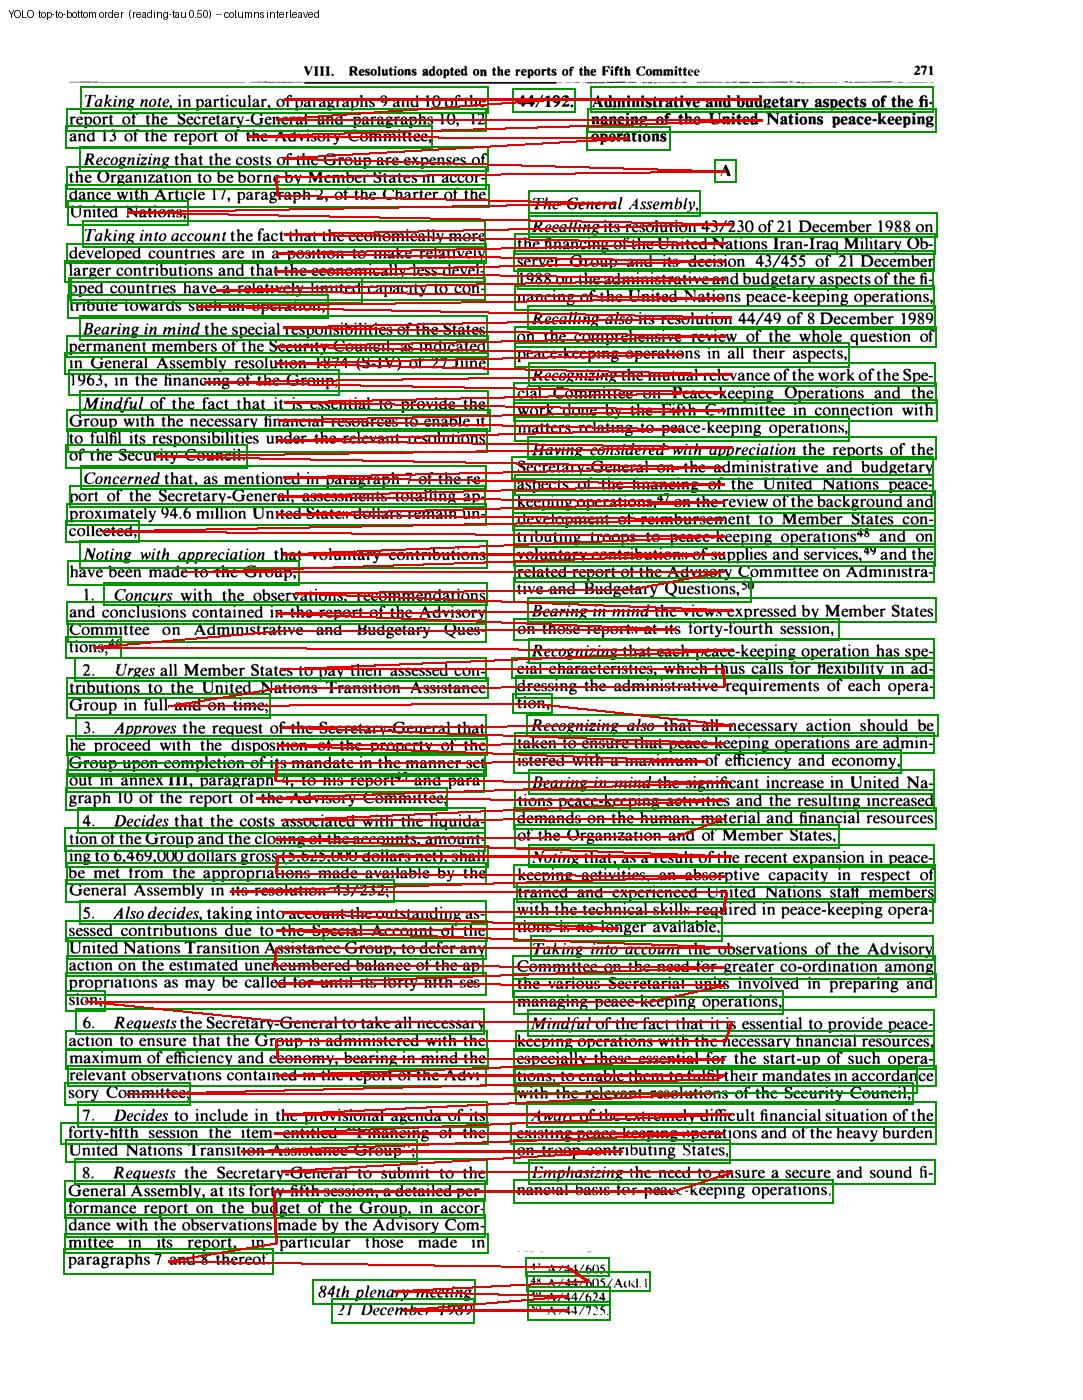
\includegraphics[width=\linewidth]{eng_yolo_order.jpg}
\caption{Box detector, top-to-bottom: \tw{}$=0.50$}\end{subfigure}\hfill
\begin{subfigure}{0.47\textwidth}\centering
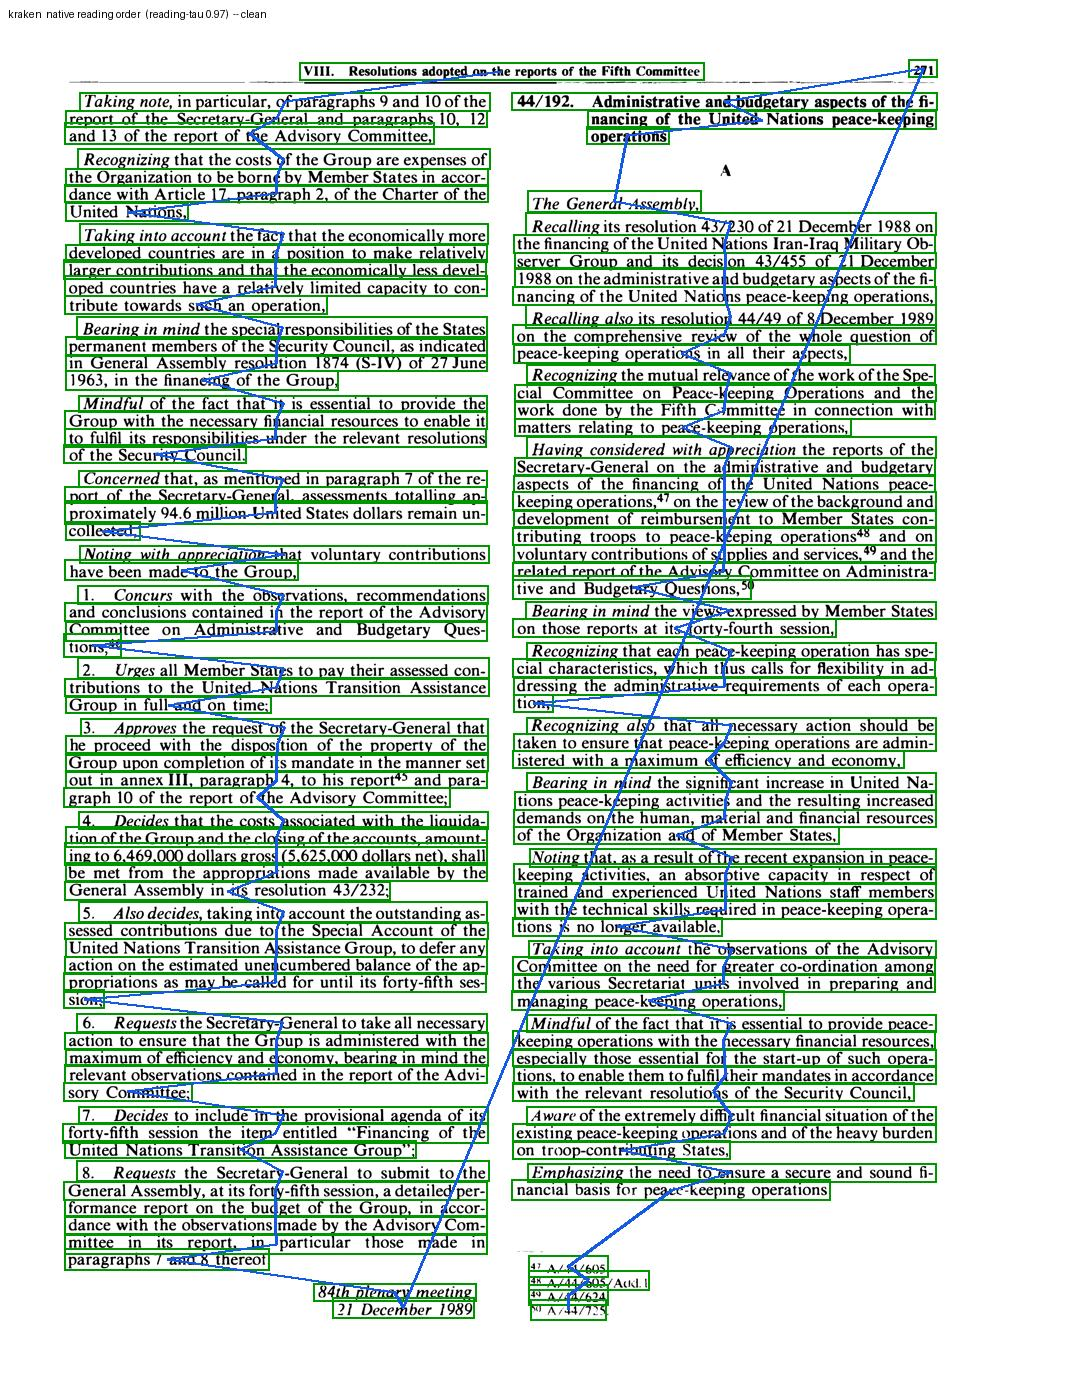
\includegraphics[width=\linewidth]{eng_kraken_order.jpg}
\caption{Layout-aware, native: \tw{}$=0.97$}\end{subfigure}
\caption{Two-column English page. Green: detected lines. Red: reading order handed
to the recogniser. Same detection, opposite order.}
\label{fig:eng}
\end{figure}

\begin{figure}[t]
\centering
\begin{subfigure}{0.47\textwidth}\centering
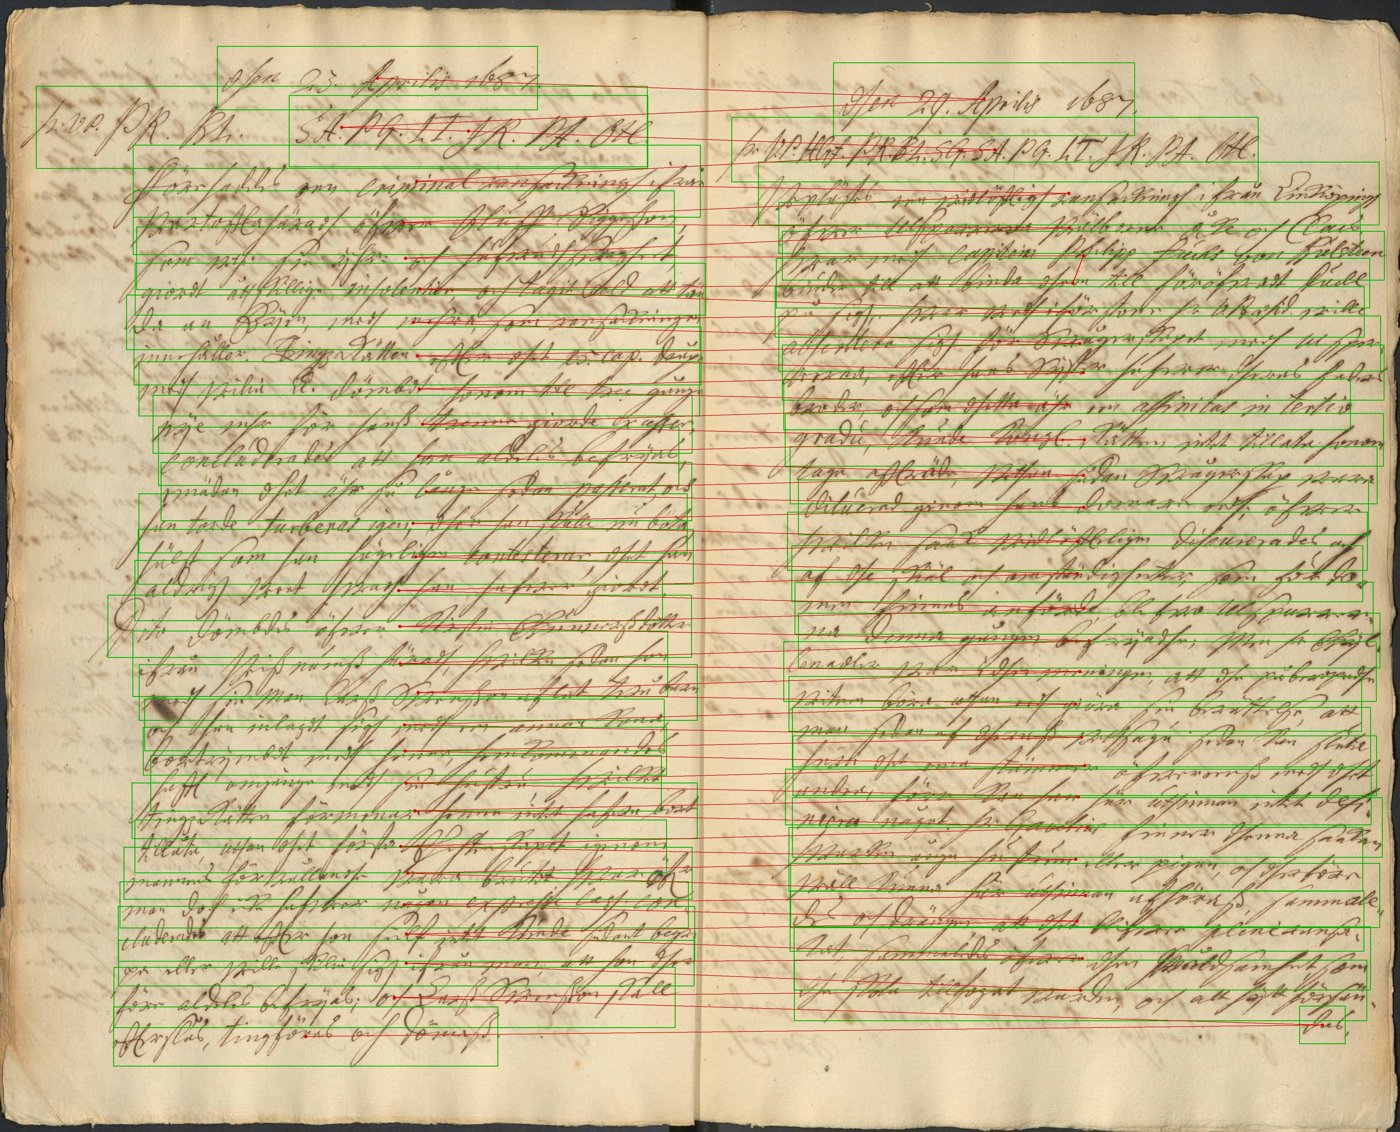
\includegraphics[width=\linewidth]{swe_yolo_order.jpg}
\caption{Box detector, top-to-bottom: \tw{}$=0.47$}\end{subfigure}\hfill
\begin{subfigure}{0.47\textwidth}\centering
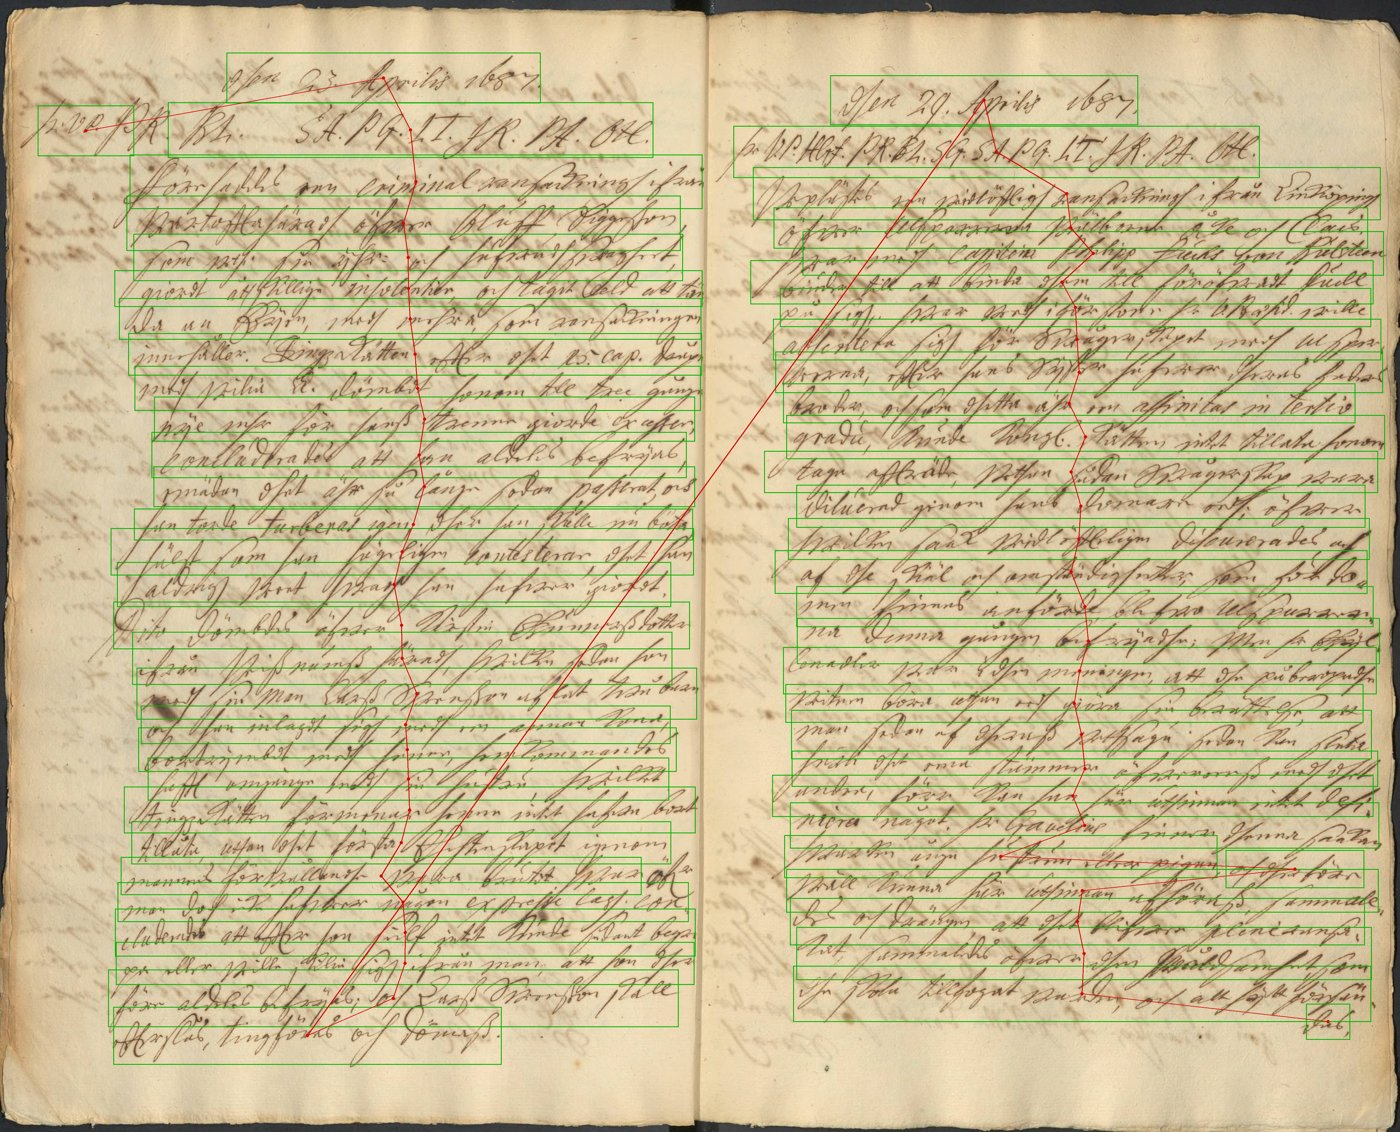
\includegraphics[width=\linewidth]{swe_kraken_order.jpg}
\caption{Layout-aware, native: \tw{}$=1.00$}\end{subfigure}
\caption{A ${\sim}$17th-century Swedish handwritten court record (Riksarkivet,
G\"ota hovr\"att). Three centuries and one script away from
Figure~\ref{fig:eng}, the same tax appears --- reading order is a function of
layout, not of date or hand.}
\label{fig:swe}
\end{figure}

\section{Recovering reading order with a cheap ordering stage}
\label{sec:recover}

The results so far show \emph{that} pure detectors lose reading order, but not
\emph{why} in a useful sense: we deliberately gave them the naive top-to-bottom
sort. The question a practitioner actually cares about is whether that gap is
intrinsic to a fast detector, or an accident of the ordering heuristic. We test
this directly by holding detection fixed --- the exact same YOLO and Surya boxes
--- and swapping only the ordering rule.

\textbf{Ordering rules.} We compare three geometric rules applied to the detected
boxes: (i) \emph{top-to-bottom}, the naive baseline; (ii) \emph{column
clustering}, which groups boxes into columns by horizontal gaps between box
centres, reads each column top-to-bottom and columns left-to-right; and (iii)
\emph{XY-cut}~\cite{xycut}, recursive projection profiling. None uses learning or
page content; all run in negligible time relative to detection.

\begin{table}[t]
\centering
\caption{Reading-order \tw{} on multi-column pages with detection held fixed;
only the ordering rule changes. Column clustering closes the gap to the
layout-aware segmenter. Means with 95\% bootstrap CIs over pages ($n=15$).}
\label{tab:ordering}
\begin{tabular}{lccc}
\toprule
Ordering on YOLO boxes & English & Swedish & Middle-Fr. \\
\midrule
top-to-bottom (naive)     & $0.50$ & $0.47$ & $0.52$ \\
XY-cut                    & $0.50$ & $0.47$ & $0.52$ \\
\textbf{column clustering}& $\mathbf{0.99}$ & $\mathbf{1.00}$ & $\mathbf{0.98}$ \\
\midrule
kraken (native, ref.)     & $0.97$ & $1.00$ & $1.00$ \\
\bottomrule
\end{tabular}
\end{table}

\textbf{A cheap ordering stage recovers the gap.} Table~\ref{tab:ordering} and
Figure~\ref{fig:ordering}(a) give the result. Column clustering lifts multi-column
\tw{} from $0.50$ $[0.47,0.54]$ to $0.99$ $[0.98,1.00]$ --- a paired gain of
$+0.49$ $[0.44,0.53]$ whose confidence interval excludes zero --- landing on the
layout-aware segmenter's $0.99$ $[0.98,1.00]$, i.e.\ statistically
indistinguishable from it. XY-cut, by contrast, does \emph{not} help here:
full-width running heads bridge the columns and defeat the vertical projection
cut, a known failure mode that centre-based clustering avoids. The reading-order
gap is therefore not intrinsic to a fast detector; it is an artefact of the
ordering heuristic, and a trivial geometric stage removes it.

\textbf{Downstream stake.} Kendall \tw{} is abstract, so we translate it into text
error. Assuming a perfect line recogniser (we substitute each detected line with
its ground-truth transcription and vary only the order), we concatenate the lines
in each system's order and measure the word error against the correctly ordered
text. Figure~\ref{fig:ordering}(b): on multi-column pages naive ordering alone
inflicts a median $82\%$ word error (Swedish $93\%$) --- a clean line-level
transcription rendered unusable purely by order --- which column clustering cuts
to $2\%$, matching kraken. On single-column pages every method stays near $2\%$.

\textbf{Scaling and cross-collection check.} To confirm the effect is not an
artefact of five pages, we scale the Swedish evaluation to $28$ pages drawn from
\emph{two} independent Riksarkivet collections --- G\"ota hovr\"att appeal-court
protocols and the Trolldomskommissionen (witchcraft-commission) records. The
result holds and tightens: reading-order \tw{} moves from $0.51$ $[0.47,0.56]$ for
naive ordering to $1.00$ $[0.99,1.00]$ for column clustering, matching kraken's
$1.00$ $[1.00,1.00]$; order-induced word error falls from $85\%$ $[77,91]$ to
$1\%$ $[0,2]$. That the same recovery appears on a second, independently produced
Swedish court-hand collection indicates the finding generalises beyond a single
archive. The same holds for the multi-column English printed material: scaled to
$8$ pages across two independent two-column UN resolution documents, naive
ordering stays at \tw{} $0.50$ $[0.50,0.51]$ while column clustering reaches
$0.99$ $[0.99,1.00]$, matching kraken ($0.98$).

\begin{figure}[t]
\centering
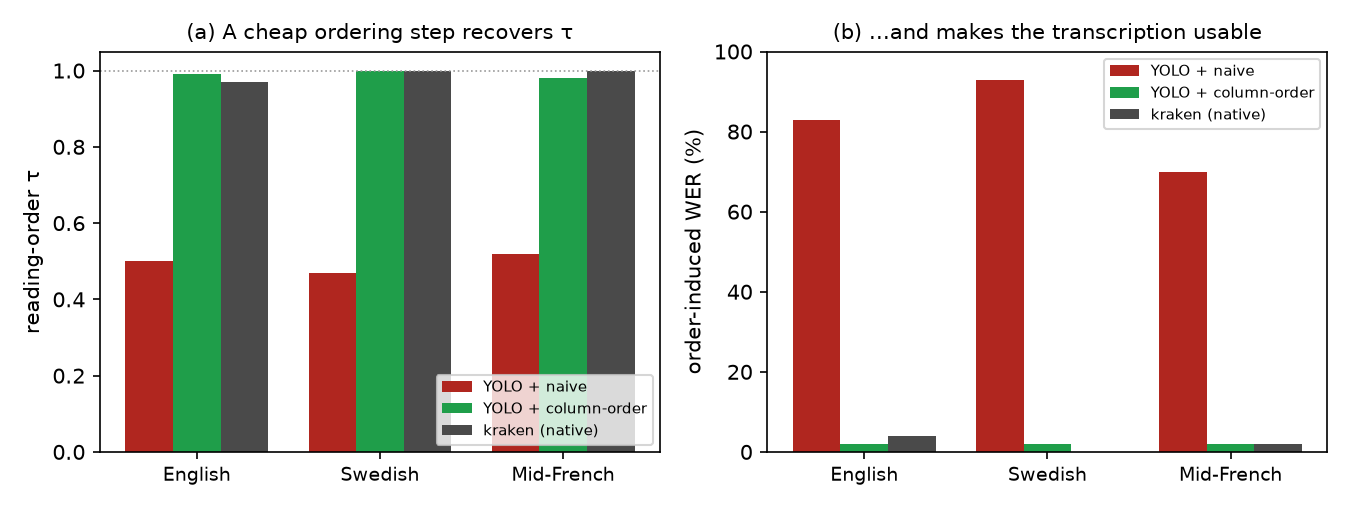
\includegraphics[width=0.92\linewidth]{ordering_control.png}
\caption{Holding detection fixed on multi-column pages. (a) A column-clustering
ordering stage on the fast detector recovers reading-order \tw{} to the
layout-aware segmenter's level. (b) The same stage cuts order-induced word error
(perfect line recognition assumed) from a median $82\%$ to $2\%$.}
\label{fig:ordering}
\end{figure}

\section{Discussion}

\textbf{Fast detection plus cheap ordering is enough.} The headline practical
finding is that one does not need a heavier layout-aware segmenter to get correct
reading order on these pages. A fast box detector, roughly nine times quicker per
page than kraken, plus a column-clustering ordering stage that costs negligible
time, matches the layout-aware segmenter on reading-order \tw{}
(Section~\ref{sec:recover}) and on the resulting text error. The heavy segmenter's
advantage over a naive detector was real but recoverable; it was the ordering
step, not the segmentation model, that mattered. The recommendation is therefore
not two-tier but simple: pair a fast detector with an explicit ordering stage,
and reserve heavier segmenters for cases the geometric rule cannot handle.

\textbf{Era-invariance.} That the same detection-versus-order split appears on a
seventeenth-century Swedish manuscript and a twentieth-century printed English
page --- about three centuries and a script apart --- indicates the effect is
driven by layout rather than by period or hand. This is what makes the finding
generalise, and why a benchmark spanning several centuries is a feature rather
than noise.

\textbf{Recognisers are not detectors.} Tesseract and docTR order well when they
detect, but on the Swedish court hand they matched $27\%$ and $0\%$ of lines
respectively. Their strong overall order numbers come from the easy printed pages,
not the hard manuscripts. Reported as an average this would flatter them; reported
per page, with the validity guard, it correctly reads as a detection failure on
historical handwriting.

\textbf{Even a commercial system is not immune.} As a spot check we ran
Transkribus (the Text Titan II super-model, via the web app) on several of the
multi-column pages. It detected lines almost perfectly and ordered the two
handwritten manuscripts flawlessly (Swedish court hand and Middle-French, \tw{}
$=1.00$), but on \emph{both} two-column printed English pages it read \emph{across}
the columns line by line, scoring \tw{} $=0.51$ and $0.50$ --- the same collapse
as the pure detectors, on the layout that looks easiest. Reading order is not
something a strong recognition model can be assumed to get for free; it depends on
the layout segmentation, and even a leading commercial system can miss it on clean
multi-column print.

\section{Limitations and honesty notes}
\label{sec:honesty}

This is a small, deliberately careful pilot, and it is easier to trust because of
what it refuses to claim. Reading order is scored only where detection succeeded
(the validity guard), so no \tw{} is computed on a handful of lines. German is
\emph{excluded from all scored tables}: its ground truth is under-annotated ---
every system, including the layout-aware ones, detects substantially more lines
than the ground truth lists --- so its F and \tw{} are not comparable, and this is
a ground-truth coverage issue rather than a system result. Five pages per language
is enough to establish the effects cleanly and with confidence intervals that
exclude the null, but not to rank systems finely; the ordering stage is evaluated
only against document-order ground truth, which is itself an editorial choice on
the hardest pages. The natural next steps are (i) scaling to dozens of pages per
language for finer ranking; (ii) datasets with explicit region and reading-order
ground truth, such as cBAD~\cite{cbad} and DIVA-HisDB~\cite{divahisdb}; (iii)
adding heavier segmenters and pipelines (Transkribus~\cite{transkribus}, Loghi
with Laypa, PaddleOCR PP-Structure) and learned reading-order models; and (iv)
reporting additional order metrics beyond Kendall \tw{} for robustness. The
downstream analysis assumes perfect line recognition to isolate ordering; a full
end-to-end study would compose real recognition error with the ordering error.

\section{Conclusion}

On historical documents, line detection is close to solved and is no longer what
separates segmentation systems; reading order is, and only on multi-column
layouts. But that gap is not intrinsic to fast detectors: a trivial
column-clustering ordering stage recovers it to the level of a heavier
layout-aware segmenter, statistically and in downstream word error, at a fraction
of the cost. The practical takeaway is to pair a fast detector with an explicit
ordering stage rather than reach for a heavier model. More broadly, we recommend
that reading order be measured and reported as a first-class metric alongside
recognition accuracy, and we release the pages, ground truth, predictions and a
reproducible scoring harness so the measurement is easy to repeat and extend.

\vspace{0.5em}
\small
\textbf{Data and code.} The benchmark --- data, ground truth, predictions and
harness --- is released openly with a per-page provenance manifest.

\begin{thebibliography}{99}
\small
\bibitem{kraken} B.~Kiessling. \emph{Kraken --- an universal text recognizer for
the humanities}. Digital Humanities Conference (DH2019), Utrecht, 2019.
\bibitem{transkribus} P.~Kahle, S.~Colutto, G.~Hackl, and G.~M\"uhlberger.
\emph{Transkribus --- a service platform for transcription, recognition and
retrieval of historical documents}. In \emph{14th IAPR ICDAR}, pp.~19--24, 2017.
\bibitem{pylaia} J.~Puigcerver. \emph{Are multidimensional recurrent layers really
necessary for handwritten text recognition?} In \emph{14th IAPR ICDAR},
pp.~67--72, 2017.
\bibitem{tesseract} R.~Smith. \emph{An overview of the Tesseract OCR engine}. In
\emph{9th ICDAR}, pp.~629--633, 2007.
\bibitem{yolov8} G.~Jocher, A.~Chaurasia, and J.~Qiu. \emph{Ultralytics YOLOv8}.
Software, 2023. \url{https://github.com/ultralytics/ultralytics}.
\bibitem{surya} V.~Paruchuri. \emph{Surya: OCR, layout analysis and reading-order
detection}. Software, 2024. \url{https://github.com/VikParuchuri/surya}.
\bibitem{doctr} Mindee. \emph{docTR: Document Text Recognition}. Software, 2021.
\url{https://github.com/mindee/doctr}.
\bibitem{htrunited} A.~Chagu\'e, T.~Cl\'erice, and L.~Romary. \emph{HTR-United:
mutualise la donn\'ee d'entra\^inement en peu de clics}. In \emph{Humanist\'ica},
2021. \url{https://htr-united.github.io/}.
\bibitem{page} S.~Pletschacher and A.~Antonacopoulos. \emph{The PAGE (Page
Analysis and Ground-truth Elements) format framework}. In \emph{20th ICPR},
pp.~257--260, 2010.
\bibitem{kendall} M.~G.~Kendall. \emph{A new measure of rank correlation}.
\emph{Biometrika}, 30(1--2):81--93, 1938.
\bibitem{xycut} G.~Nagy and S.~Seth. \emph{Hierarchical representation of optically
scanned documents}. In \emph{7th ICPR}, pp.~347--349, 1984.
\bibitem{cbad} M.~Diem, F.~Kleber, S.~Fiel, T.~Gr\"uning, and B.~Gatos.
\emph{cBAD: ICDAR2017 competition on baseline detection}. In \emph{14th IAPR
ICDAR}, pp.~1355--1360, 2017.
\bibitem{divahisdb} F.~Simistira, M.~Seuret, N.~Eichenberger, A.~Garz,
M.~Liwicki, and R.~Ingold. \emph{DIVA-HisDB: a precisely annotated large dataset
of challenging medieval manuscripts}. In \emph{15th ICFHR}, pp.~471--476, 2016.
\bibitem{dhsegment} S.~Ares Oliveira, B.~Seguin, and F.~Kaplan. \emph{dhSegment: a
generic deep-learning approach for document segmentation}. In \emph{16th ICFHR},
pp.~7--12, 2018.
\bibitem{layoutreader} Z.~Wang, Y.~Xu, L.~Cui, J.~Shang, and F.~Wei.
\emph{LayoutReader: pre-training of text and layout for reading order detection}.
In \emph{EMNLP}, pp.~4735--4744, 2021.
\end{thebibliography}

\end{document}
